\documentclass[12pt,a4paper]{article}

% Packages
\usepackage{
    amsmath,
    amssymb,
    graphicx,
    titletoc,
    fancyhdr,
    geometry,
    babel,
    xcolor,
    enumerate,
    fix-cm,
    tocbibind,
    listings,
    float,
    enumitem,
    subcaption,
    hyperref
}

% Define colors
\definecolor{vgreen}{RGB}{104,180,104}
\definecolor{vblue}{RGB}{49,49,255}
\definecolor{vorange}{RGB}{255,143,102}

% Listings customization
\renewcommand\lstlistingname{Figura}
\renewcommand\lstlistlistingname{Figura}

\makeatletter
\newcommand*\@lbracket{[}
\newcommand*\@rbracket{]}
\newcommand*\@colon{:}
\newcommand*\colorIndex{%
    \edef\@temp{\the\lst@token}%
    \ifx\@temp\@lbracket \color{black}%
    \else\ifx\@temp\@rbracket \color{black}%
    \else\ifx\@temp\@colon \color{black}%
    \else \color{vorange}%
    \fi\fi\fi
}
\makeatother

% Setup for listings
\lstset{
    captionpos=b,
    belowcaptionskip=\bigskipamount,
    frame=single,
    basicstyle=\small\ttfamily,
    numbers=left,
    numberstyle=\tiny\color{gray},
    xleftmargin=2em,
    framexleftmargin=2em,
    backgroundcolor=\color{vgreen!10},
    stepnumber=1,
    showstringspaces=false,
    keywordstyle=\color{vblue},
    commentstyle=\color{gray},
    stringstyle=\color{vorange},
}

\begin{document}

\begin{titlepage}
    \centering
    
\includegraphics[scale=1]{M2_Modelos_de_Programación/reporte/figuras/Logo_Tec.png}\\
    \vspace{.5cm}
    \bfseries\large Escuela de Ingeniería y Ciencias
        
    \vspace{5cm}
    \centering
    \textbf{\Huge Cómputo en la Nube}
    \vspace{0.5cm}
        
    {\Large Creación de una Máquina Virtual de manera Local}

    \vspace{5cm}
        
    \textbf{\LARGE Armando Bringas Corpus}
        
    \vspace{0.5cm}
        
    {\large A01200230}
        
    \vfill
        
\end{titlepage}

\section{Introducción}

Lorem ipsum

\section{Instalación de Oracle Virtual PC}

\begin{figure}[H]
    \centering
    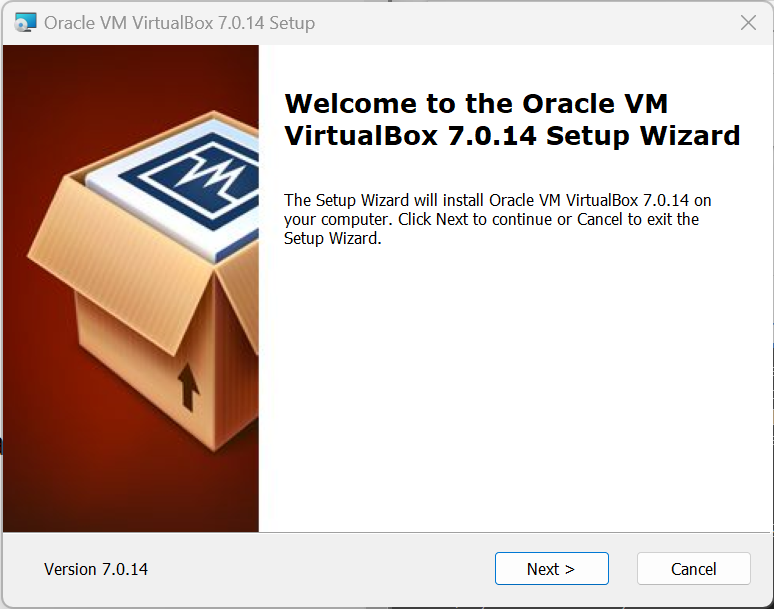
\includegraphics[width=1\linewidth]{M3_Virtualización_y_Contenedores/Tarea_2_Máquina_Virtual_Local/reporte/figuras/2-1_Instalación_Oracle_VM.png}
    \captionof{lstlisting}{Instalación de VirtualBox 7.0.14}
    \label{fig:Instalación_VirtualBox_1}
\end{figure}


\begin{figure}[H]
    \centering
    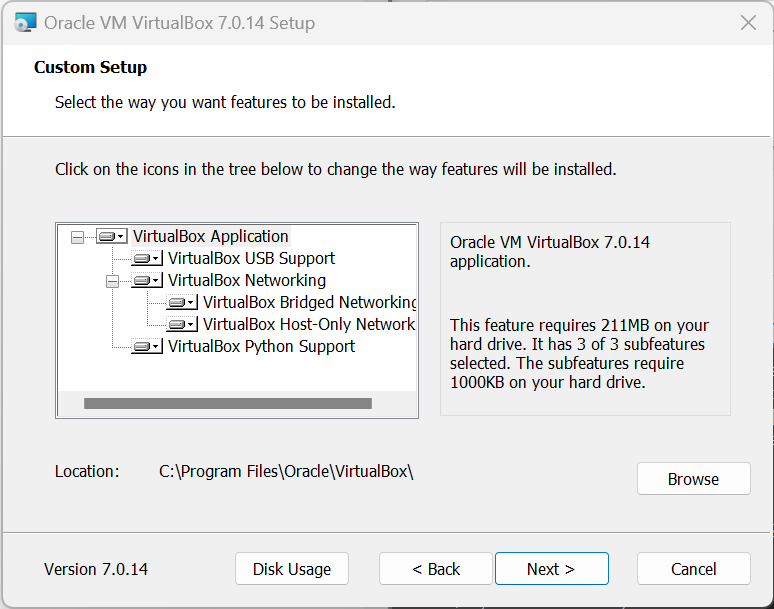
\includegraphics[width=1\linewidth]{M3_Virtualización_y_Contenedores/Tarea_2_Máquina_Virtual_Local/reporte/figuras/2-2_Instalación_Oracle_VM.png}
    \captionof{lstlisting}{Instalación de VirtualBox 7.0.14}
    \label{fig:Instalación_VirtualBox_2}
\end{figure}


\section{Creación de la Máquina Virtual de Debian}


\section{Instalación y configuración de los servicios}


\section{Personalización del sitio web}


\section{Descripción de los resultados obtenidos}


\section{Reflexión sobre las Máquinas Virtuales}


\vspace{1em}




\end{document}
